\subsection{Жизненный  цикл  программного  обеспечения  (ПО).  Основные  виды  деятельности  при  разработке  ПО. Каскадная и итерационная модели жизненного цикла.}

Весь период существования ПО, связанный с подготовкой к его разработке, разработкой, использованием и модификациями, до того момента, когда полностью прекращается всякое ее использование, называют \textbf{жизненным циклом ПО}.

Процессы жизненного цикла ПО строятся из отдельных видов деятельности (activities).
Стандартом ISO/IEC 12207 Standard for Information Technology определены 74 вида деятельности, связанной с разработкой и поддержкой ПО.
Основные из них (думаю, из этого знать нужно только выделенное, как основные типы деятельности):
\begin{itemize}
    \item \textbf{Приобретение ПО}: инициация приобретения, подготовка запроса предложений, подготовка контракта, анализ поставщиков, получение ПО и завершние приобретения.
    \item \textbf{Разработка ПО}: развертывание процесса разработки, анализ системных требований, проектирование (программно-аппаратной) системы в целом, анализ требований к ПО, проектирование архитектуры ПО, детальное проектирование, кодирование и отладочное тестирование, интеграцию ПО, квалификационное тестирование ПО, системную интеграцию, квалификационное тестирование системы, развертывание (установку или инсталляцию) ПО, поддержку процесса получения ПО.
    \item \textbf{Поддержка ПО}: развертывание процесса поддержки, анализ возникающих проблем и необходимых изменений, внесение изменений, экспертизу и передачу измененного ПО, перенос ПО с одной платформы на другую, изъятие ПО из эксплуатации.
    \item \textbf{Управление проектом}: запуск проекта и определение его рамок, планирование, выполнение проекта и надзор за его выполнением, экспертизу и оценку проекта, свертывание проекта.
\end{itemize}

\textbf{Каскадная и итерационная модели жизненного цикла ПО}

\textbf{Каскадная модель.} Основная суть \textbf{каскадной} модели в том, что этапы зависят друг от друга и следующий начинается, когда закончен предыдущий, образуя таким образом поступательное (каскадное) движение вперед. 

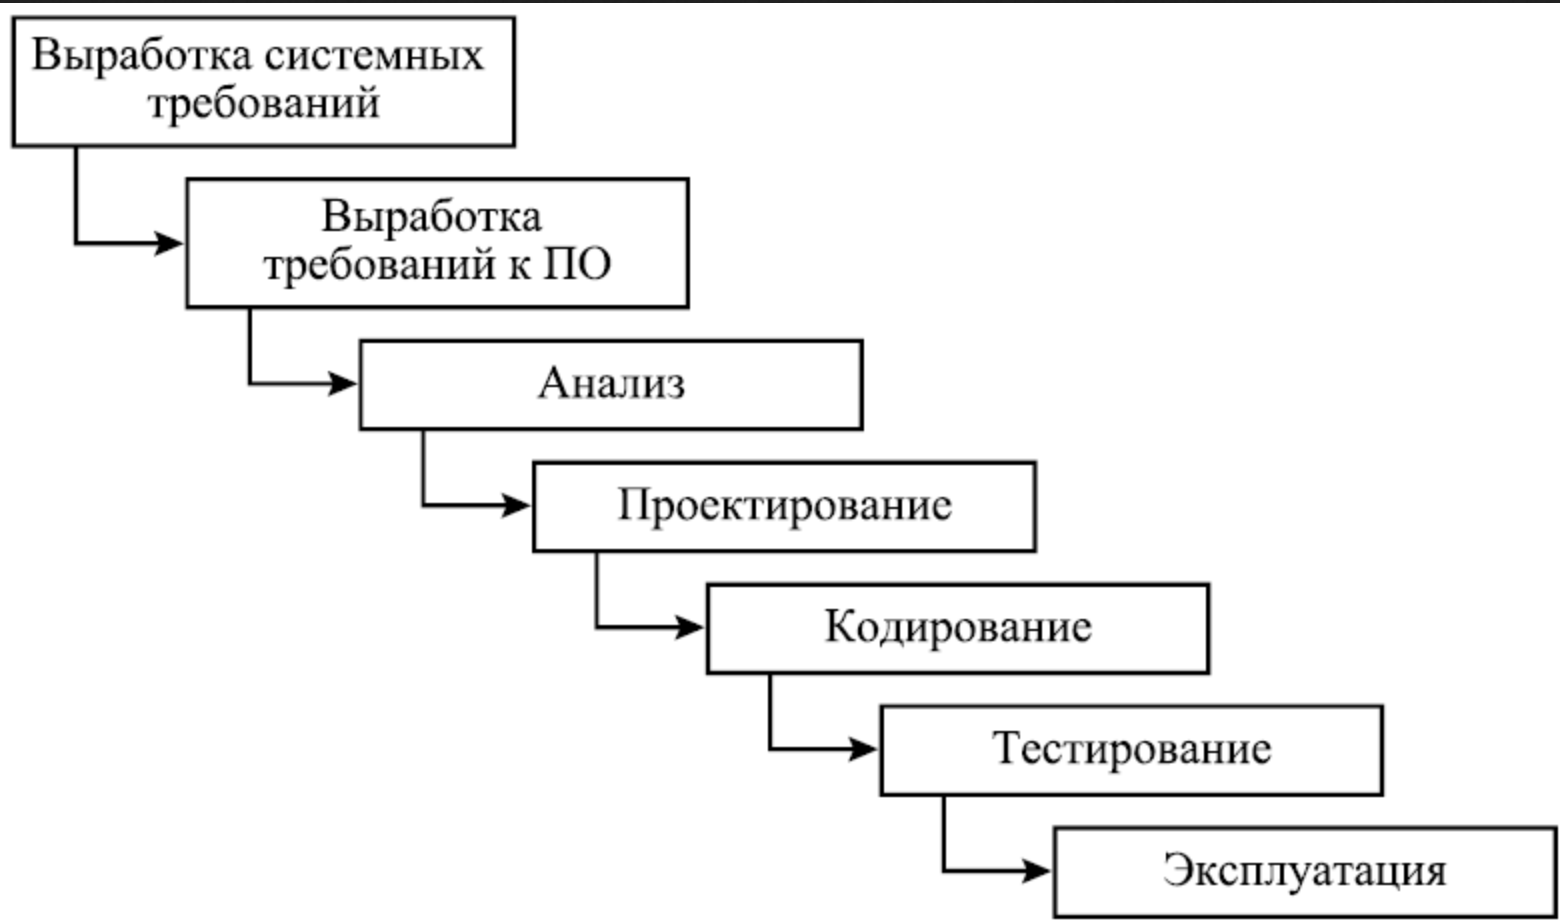
\includegraphics[width=0.24\textwidth]{pics/cascade.png}

Параллелизм этапов в каскадной модели, хоть и ограничен, но возможен для абсолютно независимых между собой работ. При этом интеграция параллельных кусков все равно происходит на каком-то следующем этапе, а не в рамках одного.

Команды разных этапов между собой не коммуницируют, каждая команда отвечает четко за свой этап.

Недостатками этой модели являются получение результата  по прохождению всех этапов и сложность выявления ошибок. Возвращаться назад трудно. Не понятно что возвращать: если произошел сбой на каком-то этапе, его последствия видны только в конце. 

Для заказчиков данная модель выглядит линейно и со стороны достаточно просто: из завершенного этапа проектирования следует программирование, а затем тестирование - и так шаг за шагом пока не будет достигнута финальная точка и цель, ради которой ведется разработка. 

Данная модель понятно и чисто укладывается в документы, например в договора и роадмапы при наличии четко обозначенных контрольных точек. В любой момент времени можно легко понять была ли пройдена та или иная точка контроля или нет, и соблюдены ли сроки. По этим причинам долговременные и особо крупные проекты, рассчитанные на десятилетия и вовлечение большого числа организаций-участников, руководствуются преимущественно каскадной моделью. 

Однако представление о простоте каскадной модели является иллюзорным. Оно появляется из-за ограниченного видения клиентом всего процесса, ведь данная модель не подразумевает вовлечение заказчика в детали процессов разработки, и демонстрирует понятный и конечный результат работы только на контрольных точках и в конце проекта. 

В реальности каскадную модель нельзя назвать простой, на практике ею сложно управлять.  Внесение заказчиком значительных изменений в процессе разработки по каскадной модели или срабатывание серьезных не предусмотренных проектом рисков несут разрушительный характер для всего процесса - модель приходиться перестраивать, графики перепланировать. 

\textbf{Итерационная модель.} Итерационная модель предполагает разбиение проекта на части (этапы, итерации) и прохождение этапов жизненного цикла на каждом их них. Каждый этап является законченным сам по себе, совокупность этапов формирует конечный результат.

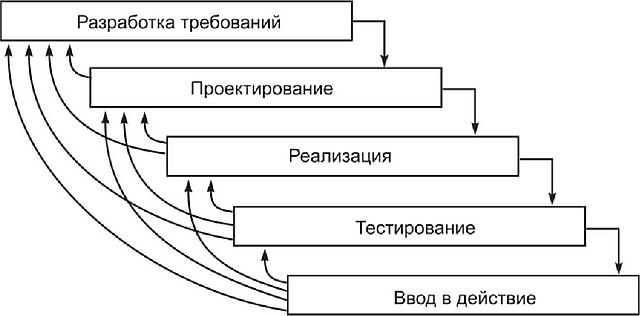
\includegraphics[width=0.24\textwidth]{pics/iterate.png}

Поясним разбиение на этапы на бытовом примере. Допустим, нам нужен стол в гостиную.

\begin{itemize}
\item На первом этапе мы сделает столешницу, ножки и скрепим их так, чтобы стол стоял.
\item На втором, укрепим и покрасим его.
\item А на третьем, накроем скатертью и купим подходящие к нему стулья.
На каждой итерации мы работали с одним и тем же продуктом и в конце каждой итерации получали результат, которым можно пользоваться (естественно, с определенными ограничениями).
\end{itemize}
С каждым этапом разработка приближается к конечному желаемому результату или уточняются требования к результату по ходу разработки, и соответственно в любой момент текущая итерация может оказаться последней или очередной на пути к завершению.

Данный подход позволяет бороться с неопределенностью, снимая ее этап за этапом, и проверять правильность технического, маркетингового или любого другого решения на ранних стадиях. 

Использование итерационной модели снижает риски глобального провала и растраты всего бюджета, получение несинхронизированных ожиданий и ошибочного понимания процессов как клиентом, так и каждым участником команды разработки. Оно также дает возможность завершения разработки в конце любой итерации (в каскадной модели вы должны прежде завершить все этапы).

% -------- source --------
\bigbreak
[\cite{evergreen}]
